\documentclass[a4j,12pt]{jarticle}

\usepackage[margin=0.5in]{geometry}
\usepackage{ascmac}
\usepackage{amsmath}
\usepackage{amssymb}
\usepackage{amsthm}
\usepackage{fancybox}
\usepackage{float}
\usepackage{subcaption}
\usepackage{mathrsfs}
\usepackage[dvips,final]{graphicx}
\usepackage{tabularx}
\usepackage{enumerate}
\usepackage{tikz}
\usetikzlibrary{positioning}

\numberwithin{equation}{section}
\newtheorem{example}{例}[section]

\newcommand{\N}{\mathbb N}
\newcommand{\R}{\mathbb R}
\newcommand{\C}{\mathbb C}
\newcommand{\bra}[1]{\langle{#1}|}
\newcommand{\ket}[1]{|{#1}\rangle}
\newcommand{\Expect}[3]{\langle {#1}|{#2}|{#3} \rangle}
\newcommand{\dev}[2]{\langle (\Delta {#1})^2 \rangle _{{#2}}}
\newcommand{\sgm}[1]{\sigma_{#1}}
\newcommand{\sgmOp}[1]{\hat{\sigma}_{#1}}
\newcommand{\hfangle}[1]{{\frac{#1}{2}}}
\newcommand{\clmnV}[2]
		{\left(
			\begin{matrix}
			 {#1}\\
			 {#2}\\
		 	\end{matrix}
		\right)
		}
\newcommand{\clmnVsan}[3]
		{\left(
			\begin{matrix}
			 {#1}\\
			 {#2}\\
			 {#3}\\
		 	\end{matrix}
		\right)
		}
\newcommand{\mtrx}[4]
	{\left(
		\begin{matrix}
		 {#1} & {#2} \\
		 {#3} & {#4} \\
		\end{matrix}
	\right)
	}
\newcommand{\inn}[2]{\langle{#1}|{#2}\rangle}
\newcommand{\itbf}[1]{\textit{\textbf{#1}}}

\newtheorem{dfn}{定義}[section]
\newtheorem{thm}{定理}[section]
\newtheorem{prop}[thm]{命題}
\newtheorem{lemma}[thm]{補題}
\renewcommand{\proofname}{\textbf{証明}}

\begin{document}
\title{Pointless Topology 勉強ノート}
\date{2024年6月13日〜}
\author{中村仁宣}
\maketitle

\section{Preliminary}
\subsection{Topology トポロジー}
Let $\mathcal{P}(X)$ denote the power set of $X$.
\begin{dfn}[Topology トポロジー]
  A \itbf{topological space} is an ordered pair $(X, \tau), \; \tau \subseteq \mathcal{P}(X)$ which satisfies the following properties
  \begin{enumerate}
  \item $\varnothing \in \tau$ and $X \in \tau$.
  \item if $U,V \in \tau$, then $U \cap V \in \tau$.
  \item if $\forall I, U_i \in \tau \text{ forall } i \in I$, then $\bigcup_{i\in I}U_i$.
  \end{enumerate}
  $\tau$ is called the \itbf{topology} of $X$.
  The members of the topology $U\in\tau$ is said to be \itbf{open} and $V \subseteq X$ is said to be \itbf{closed} if $\exists U$ open such that $V = U^c$.
\end{dfn}
\begin{dfn}
  If $X$ is a topological space and $x \in X$, a neighbourhood (abbreviated ``nhood``) od $x$ is a set $U$ which contains an open set $V$ containing $x$.
  Thus, $U$ is a nhood of $x$ iff $x \in U^{\circ}$.
  The collection $\mathscr{U}_x$ of all nhoods of $x$ is the nhood system of $x$.
\end{dfn}
\begin{dfn}[Separation Axioms 分離公理]
  A space $(X,\tau)$ is called $T_i$ ,if respectively satisfies the following conditions,
  \begin{enumerate}
  \item $T_0$: $\forall x,y \in X$ $\exists$ an open set $U \in \tau$ such that $U$ contains one of $x,y$ and not the other.
  \item $T_1$: $\forall x,y \in X$ $\exists$ a nhood of each not containing the other.
  \end{enumerate}
\end{dfn}
\begin{example}[$T_0$-space]
  $X=\{a,b\}, \tau=\{\varnothing, \{a\}, X\}$
\end{example}
\subsection{Posets, Lattices 半順序集合、束}
\begin{dfn}[Posets]
  A \itbf{partial order (半順序)} on a set $X$ is a binary relation $R \subseteq X \times X$ satisfying,
  \begin{enumerate}
  \item $\forall a, aRa$ (reflexivity, 反射律),
  \item $\forall a,b,c,\; aRb \; \& \; bRc \Rightarrow aRc$ (transitivity, 推移律),
  \item $\forall a,b,\; aRb \; \& \; bRa \Rightarrow a=b$ (antisymmetry, 反対称律).
  \end{enumerate}
  if moreover
  \begin{enumerate}
    \setcounter{enumi}{3}
  \item $\forall a,b$ either $aRb$ or $bRa$ holds,
  \end{enumerate}
  it is said to be a \itbf{linear} or \itbf{total} order.\\
  A \itbf{poset} or \itbf{partially ordered set}, $(X, \le)$ is a set with a partial order.
  If the order of a poset is linear (or total), it is called a \itbf{linearly ordered set}, \itbf{totally ordered set} or \itbf{chain}.
  A relation that satisfies only (1) and (2) is called \itbf{preorder}.
\end{dfn}
\begin{dfn}[Suprema, infima]
  A \itbf{supremum} $s$ of a subset $M \subseteq (X, \le)$ the least upper bound of $M$, that is
  \begin{enumerate}
  \item $\forall m \in M, m \le s,$
  \item $\forall m \in M, m \le x \Rightarrow s \le x$.
  \end{enumerate}
  Similarly, a \itbf{infimum} of a subset $M \subseteq (X, \le)$ the greatest lower bound of $M$.\\
  We also call a supremum a \itbf{join} and an infimum \itbf{meet} and notate $\sup M, \inf M$ or $\bigvee M, \bigwedge M$ respectively.\\
  For finite cases, we wirte $a \vee b := \sup\{a,b\}$ or $a_1 \vee \dots \vee a_n := \sup\{a_1\dots a_n\}$ and $a \wedge b := \inf\{a,b\}$ or $a_1 \wedge \dots \wedge a_n := \inf\{a_1\dots a_n\}$.
\end{dfn}
Since each $x\in X$ is both a lower and an upper bound of the empty set $\varnothing$,
\begin{equation}
  \sup\varnothing \text{ is the least element of } X
\end{equation}
and
\begin{equation}
  \inf\varnothing \text{ is the greatest element of } X
\end{equation}
We use the symbols $0$ or $\bot$ for the former and $1$ or $\top$ for the latter.\\
\begin{dfn}[Semilattices, Lattice]
  A \itbf{meet-semilattice} is a poset $X$ such that $\forall a,b \in X$ there exists an infimum $a \wedge b$.\\
  A \itbf{join-semilattice} is a poset $X$ such that $\forall a,b \in X$ there exists an supremum $a \vee b$.\\
  A \itbf{lattice} is a poset $X$ such that $\forall a,b \in X$ both an infimum $a \wedge b$ and a supremum $a \vee b$ exist.\\
  A \itbf{bounded lattice} is a poset in which all finite subsets have infima and suprema (i.e. a lattice with bottom and top).\\
  A poset is a \itbf{complete lattice} if every subset has a supremum and an infimum.
\end{dfn}
In a bounded semilattice, $\wedge$ or $\vee$ is a binary operation and satisfies the following properties,
\begin{align}
  & a \wedge a = a && a \vee a = a\\
  & a \wedge b = b \wedge a &&  a \vee b = b \vee a \\
  & (a \wedge b) \wedge c = a \wedge (b \wedge c)  && (a \vee b) \vee c = a \vee (b \vee c) \\
  & a \wedge 1 = a && a \vee 0 = a.
\end{align}
In other words, bounded semilattices are commutative monoids (semigroup with unit/identity element) in which every element is idempotent.\\
\begin{thm}
  Let $(A, \vee, 0)$ be a commutative monoid in which every element is idempotent.
  Then there exists a unique partial order on $A$ such that $a \wedge b$ is the join of $a$ and $b$, and $0$ is the least element.
\end{thm}
\begin{proof}
  If such a partial order exists,
  \begin{equation}
    a \le b \Leftrightarrow a \vee b = b.
  \end{equation}
  would be the correspondence. Now, let us verify this connection.\\
  \itbf{Reflexivity}\\
  \begin{equation}
   a \wedge a = a \Rightarrow a \le a.
  \end{equation}
  \itbf{Antisymmetry}\\
  If $a \le b$ and $b \le a$, then $b = a \wedge b = b \wedge a = a$ by commutativity.\\
  \itbf{Transitivity}\\
  If $a \le b$ and $b \le c$, then
  \begin{align*}
    a \wedge c &= a \wedge (b \wedge c) & (\because b \le c)\\
               &= (a \wedge b) \wedge c & (\text{associativity})\\
               &= b \wedge c & (\because a \le b)\\
               &= c & (\because b \le c)
  \end{align*}
  Hence, $a \le c$.\\
  \itbf{Join-uniqueness}\\
  Since $a \wedge (a \wedge b) = (a \wedge a) \wedge b = a \wedge b$, $a \le a \wedge b$.
  Similarly, $b \le a \wedge b$, so $a \wedge b$ is an upper-bound for $\{a,b\}$. For the leastness, suppose $a \le c$ and $b \le c$, then 
  \begin{align*}
    (a \wedge b) \wedge c &= a \wedge (b \wedge c)\\
                          &= a \wedge c\\
                          &= c.
  \end{align*}
  Hence, $a \wedge b \le c$.
\end{proof}
A lattice can also be defined purely algebraically in those terms,
\begin{dfn}
  A \itbf{lattice} $(L, \vee, \wedge)$ is an algebra (a set with two binary operations) that satisfy
  \begin{align*}
    \label{eq:lattice-def}
    & (L1) &  & a \wedge a = a && a \vee a = a                       &  & \text{(idempotency)}   \\
    & (L2) &  & a \wedge b = b \wedge a && a \vee b = b\vee a        &  & \text{(commutativity)} \\
    & (L3) &  & (a \wedge b) \wedge c = a \wedge (b \wedge c)       &  & (a \vee b) \vee c = a \vee (b\vee c)                 &  & \text{(associativity)} \\
    & (L4) &  & a \vee (a \wedge b) = a && a \wedge (a \vee  b) =  a &  & \text{(absorption identities)}
  \end{align*}
\end{dfn}
($L4$) is necessary for the two operations $\wedge, \vee$ to be consistent with the corresponding order $\le$.
In fact, $a\wedge b = b$ implies $a \vee b = a \vee ( a \wedge b) = a$ by ($L4$).\\
For homomorphisms (structure-preserving maps) of (semi)lattices and posets, we need to be a little bit careful since the order-preserving homomorphisms of posets does not always preserve the joins (or meets) as shown in the following example.(\cite{Stone} section 1.3 Exercise)
%---Example---%
\begin{example}
  Consider the posets $X=\{a \le c, b \le c\}$ and $Y=\{e \le g, f \le g, g \le h\}$, and a homomorphism $\phi : X \rightarrow Y$ which maps each element as in the diagram below:
\begin{figure}[H]
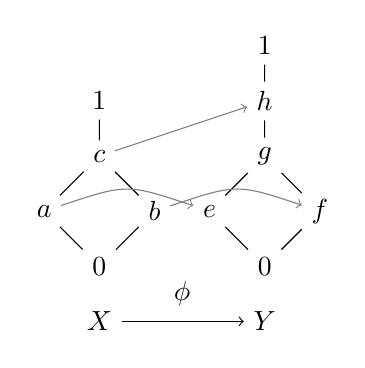
\begin{tikzpicture}[scale=.7]
  \node (one) at (0,2) {$1$};
  \node (a) at (-1,0) {$a$};
  \node (b) at (1,0) {$b$};
  \node (c) at (0,1) {$c$};
  \node (zero) at (0,-1) {$0$};
  \node (X) at (0,-2) {$X$};
  \node (one') at (3,3) {$1$};
  \node (e) at (2,0) {$e$};
  \node (f) at (4,0) {$f$};
  \node (g) at (3,1) {$g$};
  \node (h) at (3,2) {$h$};
  \node (zero') at (3,-1) {$0$};
  \node (Y) at (3,-2) {$Y$};
  \node (phi) at (1.5,-1.5) {$\phi$};
  \draw (zero) -- (a) -- (c);
  \draw (zero) -- (b) --  (c) -- (one);
  \draw (zero') -- (e) -- (g);
  \draw (zero') -- (f) --  (g) -- (h) -- (one');
  \draw[gray,->] (a) .. controls (0.5,0.5)..  (e);
  \draw[gray,->] (b) .. controls (2.5,0.5)..  (f);
  \draw[gray,->] (c) .. controls (1.5,1.5)..  (h);
  \draw[->] (X) -- (Y);
\end{tikzpicture}
\end{figure}  
Indeed, we have $a, b\le c$ and $\phi(a), \phi(b) \le \phi(c)$, which means the order is preserved, but $\phi(a \vee b) \ne \phi(a) \vee \phi(b)$.
\end{example}
(\cite{Stone} Sec.1.5) In most of the lattices we'll consider, the operations $\wedge$ and $\vee$ will satisfy an additional identity, namely the distributive law
\begin{equation}
  \label{eq:distributivity}
  \text{(i) } a \wedge (b \vee c) = (a \wedge b) \vee (a \wedge c)
\end{equation}
for all $a,b,c$.
\begin{lemma}
  If the distributive law (i) holds in a lattice, then so does its dual, i.e. the identity
  \begin{equation}
    \label{eq:ditributivity2}
    \text{(ii) } a \vee (b \wedge c) = (a \vee b) \wedge (a \vee c)
  \end{equation}
\end{lemma}
\begin{proof}
  \begin{align*}
    (a \vee b) \wedge (a \vee c) &= ((a \vee b) \wedge a) \vee ((a \vee b) \wedge c) &\text{by (i)}\\
                                 &= a \vee ((a \wedge c) \vee (b \wedge c)) &\text{by absorption law}\\
                                 &= a \vee (b \wedge c) &\text{by absorption law}
  \end{align*}
\end{proof}
Note also that in the presence of (i), we can deduce either of the two absorptive law from the other,
\begin{equation}
  a \wedge (a \vee b) = (a \wedge a) \vee (a \wedge b) = a \vee (a \wedge b)
\end{equation}
\begin{prop}
  Let $a,b,c$ be three elements of a distributive lattice $A$. Then there exists at most one $x \in A$ satisfying $x \wedge a = b$ and $x \vee a = c$.
\end{prop}
\begin{proof}
  Suppose both $x$ and $y$ satisfy the conditions. Then,
  \begin{align*}
    x &= x \wedge (x \vee a) = x \wedge c = x \wedge (y \vee a) \\
      &= (x \wedge y) \vee (x \wedge a)\\
      &= (x \wedge y) \vee b = x \wedge y
  \end{align*}
  since $b = x \wedge a = y \wedge a$ is a lower bound for $\{x,y\}$. Similarly, we have $y = x \wedge y$; so $x=y$.
\end{proof}
In any lattice, an element $x$ satisfying $x\wedge a = 0$ and $x \vee a = 1$ is called a \itbf{complement} od $a$.
The Porposition above tells us that in a distributive lattice, complements are unique when they exist.
A \itbf{Boolean algebra} is a distributive lattice $A$ equipped with an additional unary operation $\neg :A \rightarrow A$ such that $\neg a$ is a complement of $a$.
Since $\neg$ is uniquely determined by the other data in the definition, it follows that any lattice homomorphism $f:A\rightarrow B$ between Boolean algebras is actually a Boolean algebra homomorphism(i.e. commutes with $\neg$).
\begin{example}[Power set]
  For any set $X$, the power set $\mathcal{P}(X)$ of $X$ is a lattice, with $\le$ interpreted as inclusion, $\wedge$ and $\vee$ as union and intersection of subsets, and $0$ and $1$ as the empty set and the whole of $X$. Moreover $\mathcal{P}(X)$ is distributive. Since $\mathcal{P}(X)$ has complements for all its elements, it is a Boolean algebra.
\end{example}
\begin{example}[Total Order]
  Let $A$ be a totally ordered set with least and greatest elements $0$ and $1$. Then $A$ is a lattice, with $\wedge$ and $\vee$ interpreted as $\min$ and $\max$. It is distributive;
  \begin{equation}
    \min\{a, \max\{b,c\}\} = \max\{\min\{a,b\}, \min\{a,c\}\}
  \end{equation}
  But if $A$ has more than two elements, it is not a Boolean elgebra; for no element other than $0$ and $1$ can have a complement.
\end{example}
\begin{example}[Lattices of subgroups]
  Let $G$ be agroup.
\end{example}
%---Example---%
\begin{example}[Poset]
  (\cite{Gratzer} Chap.1 Exercise 4)
  Here are some examples of the possible numbers of partial orders on finite sets:\\
  \itbf{Size 1}\\
  \begin{figure}[H]
    \begin{tikzpicture}[scale=.7]
      \node (a) at (0,0) {$\circ$};
    \end{tikzpicture}
  \end{figure}
  \itbf{Size 2}\\
  \begin{figure}[H]
    \begin{tikzpicture}[scale=.7]
      \node (a) at (0,0) {$\circ$};
      \node (b) at (0,1) {$\circ$};
      \draw (a) -- (b);
    \end{tikzpicture}
  \end{figure}
  \itbf{Size 3}\\
  \begin{figure}[H]
    \begin{subfigure}{0.1\textwidth}
      \begin{tikzpicture}[scale=.5]
        \node (a) at (0,0) {$\circ$};
        \node (b) at (1,0) {$\circ$};
        \node (c) at (2,0) {$\circ$};
      \end{tikzpicture}
      \caption*{$\times 1$}
    \end{subfigure}      
    \begin{subfigure}{0.075\textwidth}
      \begin{tikzpicture}[scale=.7]
        \node (a) at (0,0) {$\circ$};
        \node (b) at (0,1) {$\circ$};
        \node (c) at (1,0.5) {$\circ$};
        \draw (a) -- (b);
      \end{tikzpicture}
      \caption*{$\times 3!=6$}
    \end{subfigure}      
    \begin{subfigure}{0.075\textwidth}
      \begin{tikzpicture}[scale=.7]
        \node (a) at (0,-1) {$\circ$};
        \node (b) at (0,0) {$\circ$};
        \node (c) at (0,1) {$\circ$};
        \draw (a) -- (b) -- (c);
      \end{tikzpicture}
      \caption*{$\times 3!=6$}
    \end{subfigure}
    \begin{subfigure}{0.11\textwidth}
      \begin{tikzpicture}[scale=.7]
        \node (a') at (-1,-1) {$\circ$};
        \node (b') at (0,0) {$\circ$};
        \node (c') at (1,-1) {$\circ$};
        \draw (a') -- (b') -- (c');
      \end{tikzpicture}
      \caption*{$\times 3$}
    \end{subfigure}
    \begin{subfigure}{0.1\textwidth}
      \begin{tikzpicture}[scale=.7]
        \node (a) at (-1,2) {$\circ$};
        \node (b) at (0,1) {$\circ$};
        \node (c) at (1,2) {$\circ$};
        \draw (a) -- (b) -- (c);
      \end{tikzpicture}
      \caption*{$\times 3$}      
    \end{subfigure}
  \end{figure}  
  \itbf{Size 4}\\
  \begin{figure}[H]
    \begin{subfigure}{0.1\textwidth}
      \begin{tikzpicture}[scale=.4]
        \node (a) at (0,0) {$\circ$};
        \node (b) at (1,0) {$\circ$};
        \node (c) at (2,0) {$\circ$};
        \node (d) at (3,0) {$\circ$};
      \end{tikzpicture}
      \caption*{$1$}
    \end{subfigure}      
    \begin{subfigure}{0.1\textwidth}
      \begin{tikzpicture}[scale=.6]
        \node (a) at (0,0) {$\circ$};
        \node (b) at (0,1) {$\circ$};
        \node (c) at (1,0.5) {$\circ$};
        \node (d) at (2,0.5) {$\circ$};
        \draw (a) -- (b);
      \end{tikzpicture}
      \caption*{$2\cdot {}_4C_2=12$}
    \end{subfigure}      
    \begin{subfigure}{0.1\textwidth}
      \begin{tikzpicture}[scale=.6]
        \node (a) at (0,0) {$\circ$};
        \node (b) at (0,1) {$\circ$};
        \node (c) at (1,0) {$\circ$};
        \node (d) at (1,1) {$\circ$};
        \draw (a) -- (b);
        \draw (c) -- (d);
      \end{tikzpicture}
      \caption*{$4!/2=12$}
    \end{subfigure}      
    \begin{subfigure}{0.075\textwidth}
      \begin{tikzpicture}[scale=.7]
        \node (a) at (0,-1) {$\circ$};
        \node (b) at (0,0) {$\circ$};
        \node (c) at (0,1) {$\circ$};
        \node (d) at (1,0) {$\circ$};
        \draw (a) -- (b) -- (c);
      \end{tikzpicture}
      \caption*{$4\cdot 3!=24$}
    \end{subfigure}
    \begin{subfigure}{0.15\textwidth}
      \begin{tikzpicture}[scale=.7]
        \node (a) at (-1,-1) {$\circ$};
        \node (b) at (0,0) {$\circ$};
        \node (c) at (1,-1) {$\circ$};
        \node (d) at (1.5,-0.25) {$\circ$};
        \draw (a) -- (b) -- (c);
      \end{tikzpicture}
      \caption*{$12$}
    \end{subfigure}
    \begin{subfigure}{0.15\textwidth}
      \begin{tikzpicture}[scale=.7]
        \node (a) at (-1,2) {$\circ$};
        \node (b) at (0,1) {$\circ$};
        \node (c) at (1,2) {$\circ$};
        \node (d) at (1.5,1.5) {$\circ$};
        \draw (a) -- (b) -- (c);
      \end{tikzpicture}
      \caption*{$12$}      
    \end{subfigure}
    \begin{subfigure}{0.1\textwidth}
      \begin{tikzpicture}[scale=.7]
        \node (a) at (0,-1) {$\circ$};
        \node (b) at (0,0) {$\circ$};
        \node (c) at (0,1) {$\circ$};
        \node (d) at (0,2) {$\circ$};
        \draw (a) -- (b) -- (c) -- (d);
      \end{tikzpicture}
      \caption*{$4\cdot 3!=24$}
    \end{subfigure}
    \begin{subfigure}{0.1\textwidth}
      \begin{tikzpicture}[scale=.7]
        \node (a) at (-1,0) {$\circ$};
        \node (b) at (0,-1) {$\circ$};
        \node (c) at (1,0) {$\circ$};
        \node (d) at (0,1) {$\circ$};
        \draw (a) -- (b) -- (c) -- (d) -- (a);
      \end{tikzpicture}
      \caption*{$2\cdot {}_4C_2=12$}
    \end{subfigure}
    \begin{subfigure}{0.1\textwidth}
      \begin{tikzpicture}[scale=.7]
        \node (a) at (-1,-1) {$\circ$};
        \node (b) at (1,-1) {$\circ$};
        \node (c) at (0,0) {$\circ$};
        \node (d) at (0,1) {$\circ$};
        \draw (a) -- (c) -- (b);
        \draw (c) -- (d);
      \end{tikzpicture}
      \caption*{$12$}
    \end{subfigure}
    \begin{subfigure}{0.1\textwidth}
      \begin{tikzpicture}[scale=.7]
        \node (a) at (1,1) {$\circ$};
        \node (b) at (-1,1) {$\circ$};
        \node (c) at (0,0) {$\circ$};
        \node (d) at (0,-1) {$\circ$};
        \draw (a) -- (c) -- (b);
        \draw (c) -- (d);
      \end{tikzpicture}
      \caption*{$12$}
    \end{subfigure}
    \begin{subfigure}{0.1\textwidth}
      \begin{tikzpicture}[scale=.7]
        \node (a) at (0,0) {$\circ$};
        \node (b) at (-1,1) {$\circ$};
        \node (c) at (0,1) {$\circ$};
        \node (d) at (1,1) {$\circ$};
        \draw (a) -- (b);
        \draw (a) -- (c);
        \draw (a) -- (d);
      \end{tikzpicture}
      \caption*{$4$}
    \end{subfigure}
    \begin{subfigure}{0.1\textwidth}
      \begin{tikzpicture}[scale=.7]
        \node (a) at (0,0) {$\circ$};
        \node (b) at (-1,-1) {$\circ$};
        \node (c) at (0,-1) {$\circ$};
        \node (d) at (1,-1) {$\circ$};
        \draw (a) -- (b);
        \draw (a) -- (c);
        \draw (a) -- (d);
      \end{tikzpicture}
      \caption*{$4$}
    \end{subfigure}
    \begin{subfigure}{0.1\textwidth}
      \begin{tikzpicture}[scale=.7]
        \node (a) at (0,0) {$\circ$};
        \node (b) at (-1,1) {$\circ$};
        \node (c) at (1,1) {$\circ$};
        \node (d) at (1,2) {$\circ$};
        \draw (a) -- (b);
        \draw (a) -- (c) -- (d);
      \end{tikzpicture}
      \caption*{$24$}
    \end{subfigure}
    \begin{subfigure}{0.1\textwidth}
      \begin{tikzpicture}[scale=.7]
        \node (a) at (0,0) {$\circ$};
        \node (b) at (-1,-1) {$\circ$};
        \node (c) at (1,-1) {$\circ$};
        \node (d) at (1,-2) {$\circ$};
        \draw (a) -- (b);
        \draw (a) -- (c) -- (d);
      \end{tikzpicture}
      \caption*{$24$}
    \end{subfigure}
    \begin{subfigure}{0.1\textwidth}
      \begin{tikzpicture}[scale=.7]
        \node (a) at (0,1) {$\circ$};
        \node (b) at (0.5,0) {$\circ$};
        \node (c) at (1,1) {$\circ$};
        \node (d) at (1.5,0) {$\circ$};
        \draw (a) -- (b) -- (c) -- (d);
      \end{tikzpicture}
      \caption*{$6!=24$}
    \end{subfigure}
    \begin{subfigure}{0.1\textwidth}
      
\begin{tikzpicture}[scale=.7]
        \node (a) at (0,1.5) {$\circ$};
        \node (b) at (0,0) {$\circ$};
        \node (c) at (1.5,1.5) {$\circ$};
        \node (d) at (1.5,0) {$\circ$};
        \draw (a) -- (b) -- (c) -- (d) -- (a);
      \end{tikzpicture}
      \caption*{${}_4C_2=6$}
    \end{subfigure}
  \end{figure}  
\end{example}
\subsection{Ideals and Filters イデアルとフィルター}
\begin{dfn}[Ideal]
  An \itbf{ideal} in a bounded distributive lattice $L$ is a subset $J \subseteq L$ such that
  \begin{eqnarray}
    \label{eq:ideal}
    && 0 \in J,\\
    && a,b \in J \Rightarrow a \vee b \in J,\\
    && b\le a \;\&\; a \in J \Rightarrow b \in J.
  \end{eqnarray}
\end{dfn}
\begin{dfn}[Filter]
  A \itbf{filter} in a bounded distributive lattice $L$ is a subset $F \subseteq L$ such that
  \begin{eqnarray}
    \label{eq:filter}
    && 1 \in F,\\
    && a,b \in F \Rightarrow a \wedge b \in F,\\
    && b \ge a \;\&\; a \in F \Rightarrow b \in F.
  \end{eqnarray}
\end{dfn}
\section{Stone Spaces}
\section{Spaces and Lattices of Open Sets}
We will suppose that all topological spaces that appear here will be $T_0$.
\subsection{Sober spaces}
\begin{dfn}[meet-irrducibility]
  Let $(X,\tau)$ be a top.space. $W\in \tau$ is said to be a \itbf{meet-irreducible} open set if $U,V\in \tau$ and $U \cap V \subseteq W$, then either $U \subseteq W$ or $V \subseteq W$.
\end{dfn}
\begin{dfn}[sober space]
  $X$ is said to be \itbf{sober} if all the meet-irreducible open sets are of the form $X\backslash \overline{\{x\}}$.
\end{dfn}
\begin{prop}
  Each Haudorff space is sober.
\end{prop}
\begin{proof}
  Suppose $W$ is meet-irreducible, for contradiction, there exists $x_1,x_2\notin W$ and $x_i \in U_i, x_j \notin U_i(i \ne j)$.
  Then $W = (W \cup U_1) \cap (W \cup U_2)$ and $W\cup U_i \nsubseteq W$.
\end{proof}

% ---REFERENCES---%
\begin{thebibliography}{10}
\bibitem[Gratzer]{Gratzer}
  George A. Gratzer, 2009, Lattice Theory: First concept and distributive lattices, Dover Publications.
\bibitem[Picado]{Picado}
  Jorge Picado, Ale\u{s} Putlr, Frames and Locales:Topology without points, Birkh\"auser.
\bibitem[Stone]{Stone}
  Peter T. Johnstone, Stone Spaces, Cambridge University Press.
\bibitem[Willard]{Willard}
  Steven Willard, General Topology, Dover Publications
\end{thebibliography}

\end{document}
